% Harbour Twin: two-page project brief for reviewers (00_START_HERE.pdf).
% Build: cd docs/brief && pdflatex start_here.tex
\documentclass[10pt,letterpaper]{article}
\usepackage[letterpaper,top=0.55in,bottom=0.6in,left=0.65in,right=0.65in,footskip=0.3in]{geometry}
\usepackage[T1]{fontenc}
\usepackage{xcolor,graphicx,titlesec,enumitem,tabularx,fancyhdr,microtype}
\definecolor{navy}{HTML}{16283B}
\definecolor{teal}{HTML}{0D5B63}
\definecolor{muted}{HTML}{5A6570}
\usepackage[hidelinks]{hyperref}
\hypersetup{pdftitle={Harbour Twin: project brief},pdfauthor={Shivaji Patil}}
\graphicspath{{../img/}}
\setlength{\parindent}{0pt}
\setlength{\parskip}{4pt}
\titleformat{\section}{\color{navy}\normalsize\bfseries\scshape}{}{0pt}{\MakeUppercase}[{\color{teal}\titlerule[0.8pt]}]
\titlespacing*{\section}{0pt}{7pt}{4pt}
\setlist[itemize]{leftmargin=12pt,itemsep=1pt,topsep=1pt,parsep=0pt,label={\color{navy}\textbullet}}
\newcommand{\num}[1]{{\color{teal}\textbf{#1}}}
\newcommand{\figcap}[1]{\par\vspace{1pt}{\color{muted}\footnotesize #1}\par}
\pagestyle{fancy}\fancyhf{}\renewcommand{\headrulewidth}{0pt}
\fancyfoot[L]{\color{muted}\footnotesize Harbour Twin \enspace$|$\enspace Shivaji Patil \enspace$|$\enspace shivaji@shivajipatil.com}
\fancyfoot[R]{\color{muted}\footnotesize \thepage/2}

\begin{document}
\noindent\fboxsep=0pt\colorbox{navy}{\parbox{\textwidth}{\centering\vspace{8pt}%
  {\color{white}\fontsize{20}{24}\selectfont\scshape\textbf{Harbour Twin}}\\[3pt]
  {\color{white!82!navy}\footnotesize\textbf{A MARITIME DIGITAL TWIN FROM PUBLIC DATA: AIS, SENTINEL-1 SAR, LIDAR AND TIDES}}\vspace{7pt}}}\\[-1pt]
{\color{teal}\rule{\textwidth}{1.6pt}}\par\vspace{2pt}

Harbour Twin builds a 3D twin of a harbour (Vancouver and St.\ John's so far) entirely from public data, and checks every product automatically. It records live AIS vessel traffic, detects ships in Sentinel-1 radar and cross-checks them against AIS, measures building heights from lidar, aligns every height to the right vertical datum, and plans for coastal floods. A Python pipeline produces the products; a CesiumJS viewer shows them. Built by Shivaji Patil in October 2026, with an AI coding agent writing much of the code under my direction and every output verified by tests and visual review.

\section{SAR ship detection, cross-checked against AIS}
\begin{minipage}[t]{0.56\textwidth}\vspace{0pt}
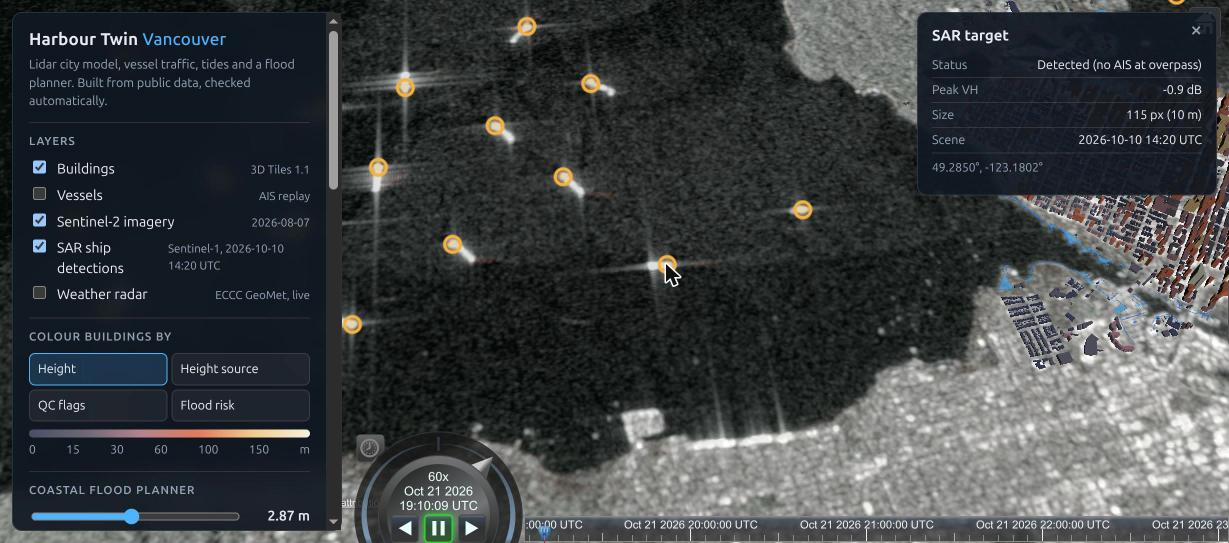
\includegraphics[width=\linewidth]{sar.jpg}
\figcap{Viewer: Sentinel-1 backscatter over English Bay, 10 Oct 2026 14:20 UTC. Rings are detected targets; one is selected.}
\end{minipage}\hfill
\begin{minipage}[t]{0.41\textwidth}\vspace{0pt}\small
\begin{itemize}
\item Sentinel-1 RTC found through the Planetary Computer STAC API and read by window, VV/VH or HH/HV.
\item Two-parameter \textbf{CFAR} on cross-pol dB over an OpenStreetMap open-water mask; bridges and piers excluded.
\item \num{77 targets} in the Vancouver scene, including the anchored freighters in English Bay; \num{12} off St.\ John's.
\item Each target is matched one-to-one to AIS interpolated to the overpass, with a gate that widens with speed for SAR azimuth shift. Radar-only targets become \textbf{dark-vessel candidates for review}.
\item \textit{Status:} matching is tested on synthetic data; the bundled AIS capture misses the satellite passes. A capture across the 22 Oct pass gives the first real cross-check.
\end{itemize}
\end{minipage}

\vspace{3pt}
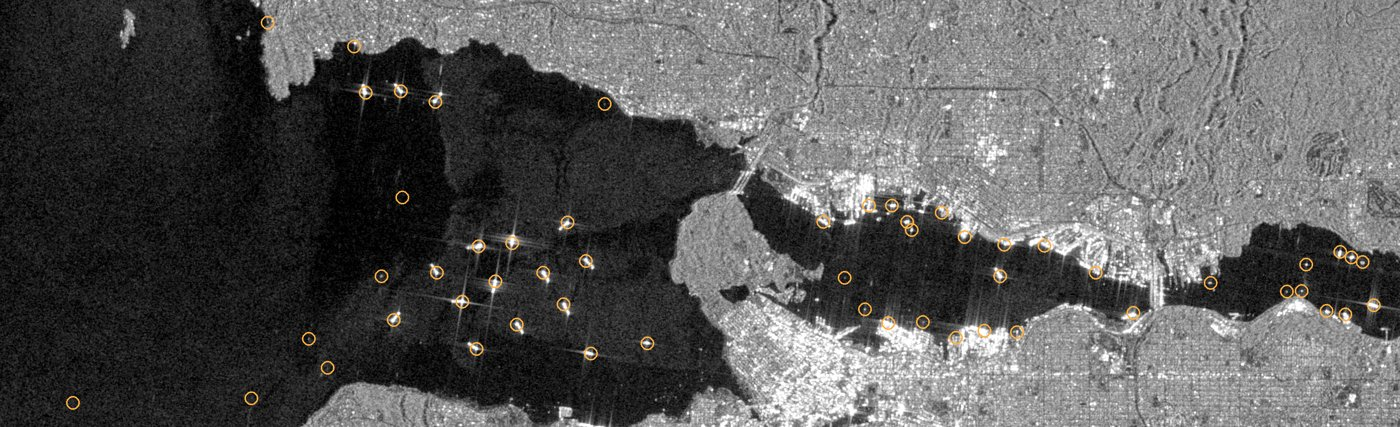
\includegraphics[width=\textwidth]{sar_detections_qc.jpg}
\figcap{Detector QC: all 77 targets ringed on the radar image (English Bay left, Burrard Inlet right). This review caught a false alarm on the Lions Gate Bridge, now masked.}

\section{Live AIS, replayed with the tide}
\begin{minipage}[t]{0.47\textwidth}\vspace{0pt}
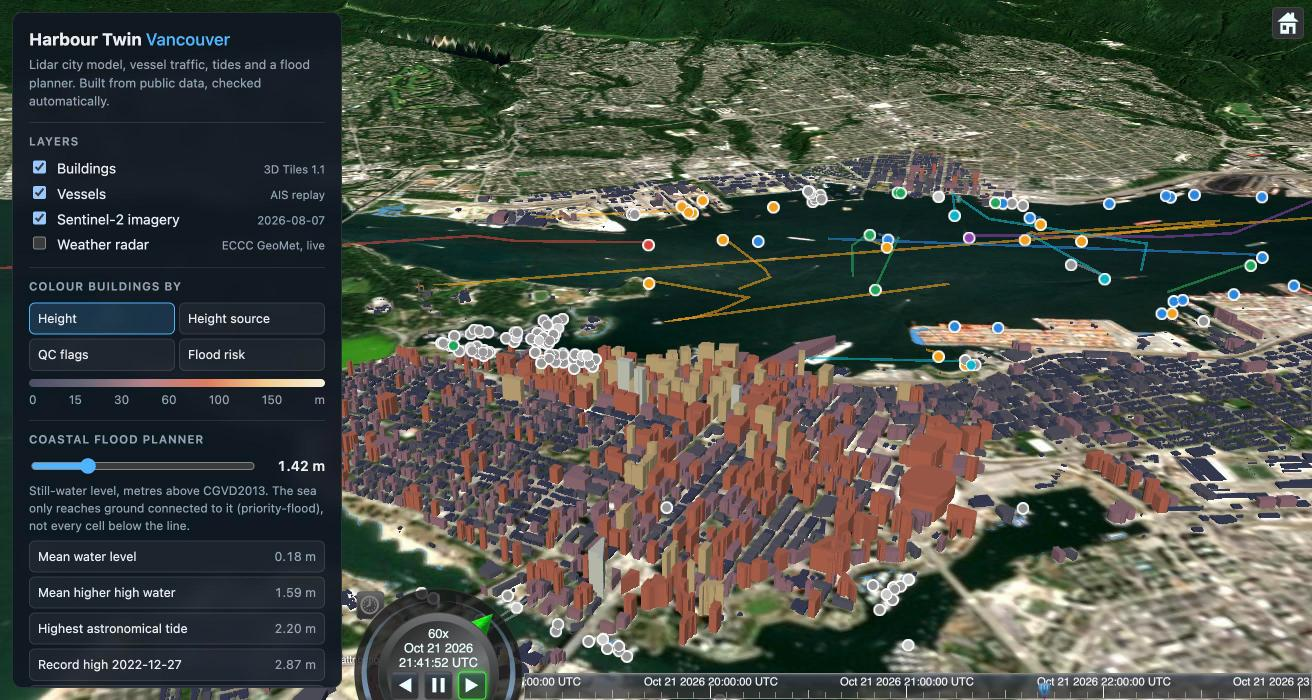
\includegraphics[width=\linewidth]{hero.jpg}
\end{minipage}\hfill
\begin{minipage}[t]{0.5\textwidth}\vspace{0pt}\small
\begin{itemize}
\item 4-hour live capture from aisstream.io: \num{347 vessels}, \num{7,854} cleaned positions, \num{769} track segments.
\item Cleaning drops impossible jumps (over 45 kn), null-island fixes and duplicates, and splits tracks on 20-minute gaps.
\item Replayed as CZML on one clock with the CHS-observed tide, so the water level and the vessels move together.
\item Lidar buildings coloured by height: \num{98.7\%} of 5,848 heights measured from lidar, published as OGC 3D Tiles 1.1 (all 69 tiles pass the Khronos validator).
\end{itemize}
\end{minipage}

\newpage
\section{What the automated checks found}
\begin{tabularx}{\textwidth}{@{}>{\raggedright\arraybackslash}p{0.27\textwidth}X@{}}
\textbf{PROJ's default datum transform is a ballpark} & CGVD2013 to WGS 84 through PROJ's automatic choice is off by \num{0.30 m} in Vancouver and \num{1.05 m} in St.\ John's (it skips the NAD83(CSRS) frame step). Explicit pipelines fix it; a regression test pins it.\\[3pt]
\textbf{The datum chain is right} & NRCan MRDEM-30 against lidar on flat ground: bias \num{0.02 m}, LE90 \num{0.69 m}. Copernicus GLO-30 handed to Cesium without a geoid correction: bias \num{+16.52 m}, and both spec gates fail, as they must.\\[3pt]
\textbf{Published building heights are often wrong} & Lidar recovers the towers (Hyatt 196.9 m vs 201 published) and catches outliers such as the 190.8 m Paradox tower tagged 10 m in OSM. \num{717} disagreements are flagged for review, not overwritten.\\[3pt]
\textbf{A second city broke two assumptions} & St.\ John's revealed a missing dependency and a CHS tide station with no CGVD2013 offset; its chart datum is now derived through the CGG2013a geoid (\num{$-$1.22 m}) and cross-checked against CGVD28.\\[3pt]
\textbf{Reads were 900$\times$ too big} & rasterio's WarpedVRT ignores COG overviews; selecting the overview explicitly cut a QC run from over 10 minutes to 16 s.\\
\end{tabularx}

\section{Coastal flood planner}
\begin{minipage}[t]{0.5\textwidth}\vspace{0pt}
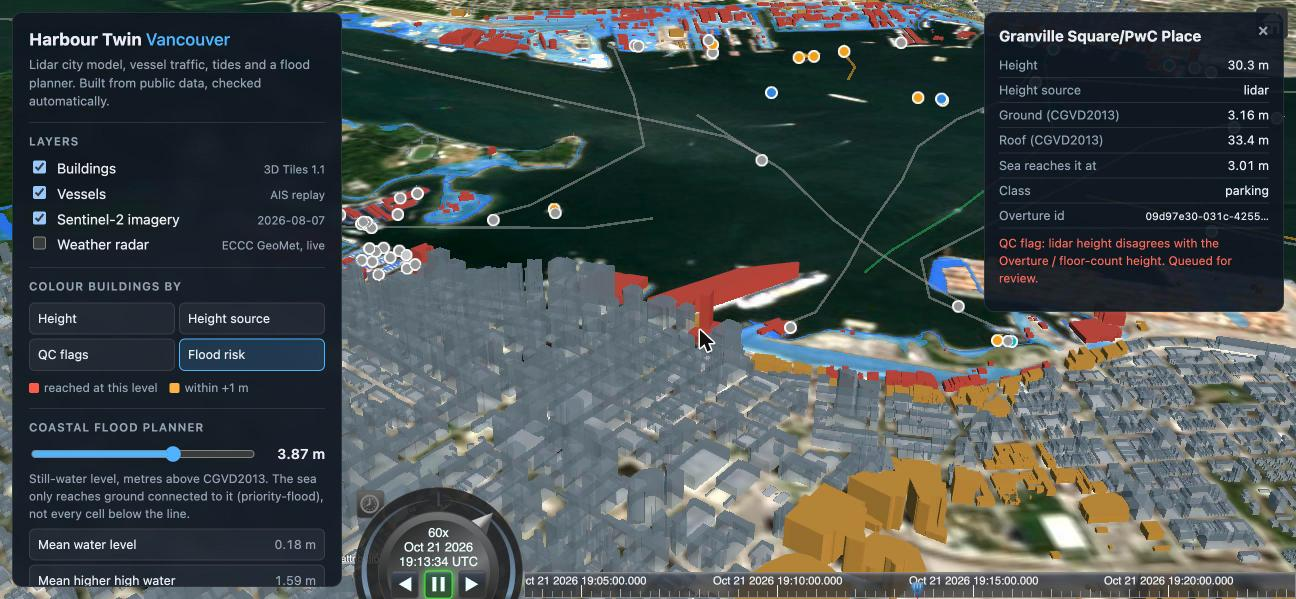
\includegraphics[width=\linewidth]{flood.jpg}
\end{minipage}\hfill
\begin{minipage}[t]{0.47\textwidth}\vspace{0pt}\small
Priority-flood gives the still-water level at which the sea actually \emph{reaches} each building over the terrain, not a bathtub threshold. Presets come from CHS station levels converted to CGVD2013.\par\vspace{3pt}
\begin{tabular}{@{}lrr@{}}
\textbf{Vancouver level} & \textbf{m} & \textbf{buildings}\\
Mean higher high water & 1.59 & 97\\
Record, 27 Dec 2022 & 2.87 & 152\\
Record + 1 m & 3.87 & 461\\
Record + 2 m & 4.87 & 938\\
\end{tabular}\par\vspace{3pt}
{\footnotesize A planning screen, not a hydrodynamic model: no waves, duration or drainage.}
\end{minipage}

\section{How it is built}
\small
\begin{minipage}[t]{0.485\textwidth}
\begin{itemize}
\item \textbf{Integrate first.} Every input is someone else's maintained product, found through STAC or its own API: NRCan lidar, Copernicus DEM, Sentinel-1/-2, Overture Maps, aisstream.io, CHS.
\item \textbf{Read only what is needed.} Windowed COG reads and DuckDB queries on GeoParquet; nothing is bulk-downloaded, and a harbour rebuilds in minutes.
\item \textbf{Every height carries its datum}: EGM2008, CGVD2013, WGS 84 or EGM96, converted only through explicit PROJ pipelines.
\end{itemize}
\end{minipage}\hfill
\begin{minipage}[t]{0.485\textwidth}
\begin{itemize}
\item \textbf{Checked:} 67 unit and acceptance tests, the Khronos glTF validator, spec gates on every elevation product, and STAC lineage back to the upstream items.
\item \textbf{One YAML per city.} St.\ John's was added with one config file; the same tests run against its products.
\item \textbf{Open formats and services:} 3D Tiles 1.1, CityJSON 2.0 (validated), DTED Level 2 and GeoPackage; a Docker image that publishes to S3-compatible object storage, with OGC API -- Features and STAC Browser via \texttt{docker compose}. Diagrams are in \texttt{docs/ARCHITECTURE.md}.
\end{itemize}
\end{minipage}
\normalsize

\section{Where to look}
\small
\begin{tabularx}{\textwidth}{@{}>{\raggedright\arraybackslash}p{0.33\textwidth}X@{}}
\texttt{docs/ARCHITECTURE.md} & Steps, modules, datums, the SAR method and its limits, tests\\
\texttt{twin/sar.py} & Sentinel-1 search, CFAR detector, AIS interpolation and matching\\
\texttt{twin/ais.py}, \texttt{twin/datum.py} & AIS capture and cleaning; explicit vertical-datum pipelines\\
\texttt{data/vancouver/QC\_REPORT.md} & The full elevation QC report the pipeline writes\\
\texttt{README.md} & Running it: \texttt{make setup data test serve}, then open \texttt{127.0.0.1:8765}\\
\end{tabularx}
\end{document}
